\chapter{Deep Learning Fundamentals}

\section{Artificial Neural Networks}

Artificial neural networks (ANNs) are a class of machine learning algorithms
that are loosely inspired by the structure of biological nervous
systems.
To be precise, each ANN consists of a collection of artificial neurons
that are connected with each other. The neurons are able to exchange
information along their connections.
A common way to arrange artificial neurons within a network is to organize
them in layers as depicted in \fref{fig:basic-network}.
\begin{figure}[h]
  \centering
  \resizebox{0.75\textwidth}{!}{\begin{neuralnetwork}[height=5]
  \tikzstyle{input neuron}=[neuron, draw, fill=white]
  \tikzstyle{hidden neuron}=[neuron, draw, fill=white]
  \tikzstyle{output neuron}=[neuron, draw, fill=white]
  \tikzstyle{link} = [->, shorten <=0pt, node distance=\nn@layerspacing, thin, draw=black];
  \inputlayer[count=4, bias=false, title=Input\\layer]
  \hiddenlayer[count=5, bias=false, title=Hidden\\layer] \linklayers
  \outputlayer[count=3, title=Output\\layer] \linklayers
\end{neuralnetwork}
}
  \caption{The structure of an ANN can be described by a
    directed graph. The nodes represent the
    neurons, the edges represent their connections, also indicating
    the flow of information.}
  \label{fig:basic-network}
\end{figure}

When an artificial neuron receives a signal on some of its
incoming connections, it may elect to become active based on the input
it collects.\footnote{The
  details of this
  process are further illustrated in \fref{sec:artificial-neurons}.}
In this state it also influences all neurons it has an outgoing
connection to by passing a signal along their
channel. Those other neurons in turn may also elect to become
active - this way a signal can propagate through the network along
the connecting edges.

Usually, each ANN consists of at least one layer of neurons that is
responsible for receiving signals from the environment - we call this
an \textit{input layer} (see \fref{fig:basic-network}). When these neurons
receive a signal from the environment, they propagate it to their
connected neighbors in the next layer. This process repeats until the
\textit{output layer} is reached. The neurons in this layer represent the
output of the whole network. Each layer in between is called a \textit{hidden
layer} because there is no direct communication between the neurons in
this layer and the environment. Networks that satisfy this basic
architectural model where each layer is fully connected with its
following layer and signals only flow in one direction without cycles
are called
\textit{fully connected feedforward networks}.

The goal behind this procedure usually is to convert an input signal
into a meaningful output by feeding it through the network. If the
network is able to detect relevant features or patterns in the input
signal, it can be used to perform tasks such as classification or
regression (i.e. approximate discrete or continuous functions).
In order for this to be possible, some kind of learning has to take
place which enables the network to capture the essence of the data it
is confronted with. We will take a further look at these aspects as
well as the mathematical model of a neural network in the following
sections.

\subsection{Modeling Artificial Neurons}
\label{sec:artificial-neurons}
To fully understand how each neuron processes the signals it receives,
it is necessary to develop a mathematical model that describes all the
operations taking place. The following descriptions are partially
based on the explanations that are provided in \cite{Haykin}.\footnote{See
  chapter I.3: \textit{Models of a Neuron} for more details.}
As shown in \fref{fig:single-neuron}, each artificial neuron
basically consists of three components:
\begin{enumerate}
  \item \textbf{A set of weighted inputs:} Each connection that is
    leading into the neuron has a weight \(w_{kj}\) associated with it
    where \(k\) denotes the neuron in question and \(j\) denotes the
    index of the neuron that delivers its input to the current neuron
    \(k\).\footnote{There might arise the question why the indexing of
    a weight from neuron \(j\) to neuron \(k\) is \(w_{kj}\) and
    \textit{not} \(w_{jk}\). This is the case because the weights are
    usually stored in matrices where each row corresponds to a
    neuron \(k\) and each column corresponds to an input \(j\) which
    allows for much faster computations by heavily utilizing
    matrix-multiplication.} The signal that
    passes the connection is multiplied by the
    related weight of that connection before arriving at the next
    component.
  \item \textbf{A summation unit:} This component adds up all the
    weighted signals that arrive at the neuron as well as a constant
    bias value
    \(b_k\) that is independent of the inputs.
  \item \textbf{An activation function:} The activation function
    \(\phi(\cdot)\) takes the output of the summation unit and applies
    a transformation to it that is usually non-linear. The value of
    the activation function is the output of the neuron which will
    travel further through the network alongside the corresponding
    connections. In \fref{sec:activation-functions}, a more
    detailed explanation of activation functions as well as some
    commonly used examples will be provided.
\end{enumerate}
\begin{figure}[h]
  \centering
  \includegraphics[width=\textwidth]{../figures/single_neuron}
  \caption{The components of a single artificial neuron. This neuron
    \(k\) receives three input signals that are first multiplied by
    the associated weights, summed up including a bias and then fed
    into an activation function that will determine the ouput signal.}
  \label{fig:single-neuron}
\end{figure}
Transforming this model into mathematical equations, the output of the
summation unit of a particular
neuron \(k\) with \(n\) input signals \(x_j\) can be described by the
following formula:
\begin{equation}
  z_k = \sum_{j=1}^{n}{x_j \cdot w_{kj}} + b_k
\end{equation}
where \(b_k\) denotes the bias term of neuron \(k\) and \(z_k\) describes the
result of the summation unit.

As a consequence, the output signal \(y_k\) of neuron \(k\) can be computed by
applying the activation function \(\phi(\cdot)\) to the output of the
summation unit which can be described by the following expression:
\begin{equation}
  y_k = \phi(z_k)
\end{equation}

\subsection{Activation Functions}
\label{sec:activation-functions}
The basic task of an activation function is to determine the level of
activity that a neuron emits based on the input it receives. Because the
incoming signals are first weighted and summed up by the summation unit, they
arrive at the activation function as a single value \(z\). Since the
output \(y\)
of the neuron is also a scalar, each activation function can be
described as \(\phi: \mathbb{R} \rightarrow \mathbb{R}\). In the
following paragraphs, an overview of the most popular activation
functions will be presented that is based on the descriptions found in
\cite{Patterson}.\footnote{See section \textit{Activation Functions}
  in chapter two.}

\paragraph{The Sigmoid Function}
This activation function transforms an input \(z\) into a range between 0
and 1 based on the following equation:
\begin{equation}
  \phi(z) = \frac{1}{1 + e^{-\theta \cdot z}}
\end{equation}
The \(\theta\) parameter is used to adjust the sensitivity of the
sigmoid function with respect to its input signal. High values of \(\theta\) lead
to steep slopes around \(z=0\) while smaller values will lead to smoother
slopes. An illustration of this relationship is presented in \fref{fig:sigmoid}.
\begin{figure}[h]
  \centering
  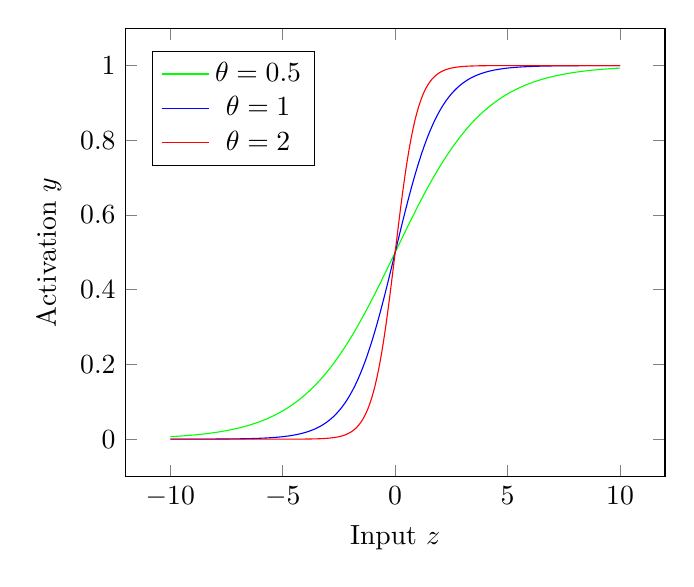
\begin{tikzpicture}
  \begin{axis}[
      xlabel={Input \(z\)},
      ylabel={Activation \(y\)},
      legend style={
        at={(0.05, 0.95)},
        anchor=north west
      }
    ]
    \addplot[green, domain=-10:10, samples=400]{1/(1+exp(-0.5*x))};
    \addplot[blue, domain=-10:10, samples=400]{1/(1+exp(-x))};
    \addplot[red, domain=-10:10, samples=400]{1/(1+exp(-2*x))};
    \legend{\(\theta = 0.5\), \(\theta = 1\), \(\theta = 2\)}
  \end{axis}
\end{tikzpicture}

  \caption{The sigmoid activation function plotted with different
    values of \(\theta\).}
  \label{fig:sigmoid}
\end{figure}

One important reason why the sigmoid function is often used is that it reduces
the impact of outliers in the data without removing them. When the
input of a neuron is large, it is reduced to a number near one, when it
is very negative, the activation evaluates to a number near zero. This
behaviour adds to the overall robustness of the network.

\paragraph{The Rectified Linear Unit (ReLU)}
Because it is not always desirable to reduce large signals to a
smaller scale, this function will only replace negative values with
zero and leave positive values untouched. This behaviour can be
modeled by the following expression:
\begin{equation}
  \phi(z) = \max(0, z)
\end{equation}
When building deep neural networks, one of the problems that sometimes
arise is that a signal will fade out when propagating through many
hidden layers. This issue is remedied to some degree by using the ReLU
function because large signals are not cut down. Due to the negative
values being set to zero, the ReLU function is also non-linear when
taking its whole domain into account. This is an important concept
because non-linear activation functions are essential for a network to
learn complex relationships. Another benefit of the ReLU function is
that its derivative is either 1 or 0. This will be important when
looking into the training of a neural network. Because of all these benefits,
ReLUs are one of the state of the art activation functions in deep
neural networks. A plot of the ReLU function is given in \fref{fig:relu}.
\begin{figure}[h]
  \centering
  \begin{tikzpicture}
  \begin{axis}[
      xlabel={Input \(z\)},
      ylabel={Activation \(y\)},
      legend style={
        at={(0.05, 0.95)},
        anchor=north west
      }
    ]
    \addplot[blue, domain=-10:10]{max(0, x)};
  \end{axis}
\end{tikzpicture}

  \caption{The ReLU activation function.}
  \label{fig:relu}
\end{figure}

\section{The Backpropagation Algorithm}

\section{Deep Networks}
